\subsection*{The Cartesian Plane}
In \typeu Activity~\ref*{PA:equationwith2vars}, we sketched the graph of the equation  $2x + 3y = 12$ in the $xy$-plane.  This $xy$-plane, with which you are familiar, is a representation of the set  $\mathbb{R} \times \mathbb{R}$ \label{sym:cartplane} or  $\mathbb{R}^2 $.  This plane is called the \textbf{Cartesian plane.}
\index{Cartesian plane}% 

The basic idea is that each ordered pair of real numbers corresponds to a point in the plane, and each point in the plane corresponds to an ordered pair of real numbers.  This geometric representation of  $\mathbb{R}^2 $ is an extension of the geometric representation of  $\mathbb{R}$ as a straight line whose points correspond to real numbers.

Since the Cartesian product  $\mathbb{R}^2 $ corresponds to the Cartesian plane, the Cartesian product of two subsets of  $\mathbb{R}$  corresponds to a subset of the Cartesian plane.  For example, if  $A$  is the interval  $\left[ {1,3} \right]$, and  $B$  is the interval  $\left[ {2,5} \right]$, then
\[
A \times B = \left\{ {\left( {x, y} \right) \in \mathbb{R}^2 \mid 1 \leq x \leq 3\text{ and }2 \leq y \leq 5} \right\}\!.
\]
A graph of the set  $A \times B$ can then be drawn in the Cartesian plane as shown in Figure~\ref{fig:cartprod}.
%\begin{figure}[h]
%\begin{center}
%\includegraphics[6.5cm,5cm]{figcartprod.bmp}
%\caption{Cartesian Product $A \times B$} \label{fig:cartprod}
%\end{center}
%\end{figure}
%
\begin{figure}[h]
\begin{center}
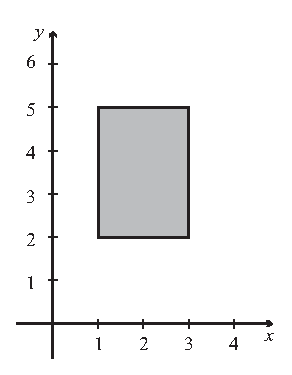
\includegraphics{figps-cartprod.eps}
\caption{Cartesian Product $A \times B$} \label{fig:cartprod}
\end{center}
\end{figure}

This illustrates that the graph of a Cartesian product of two intervals of finite length in  $\mathbb{R}$ corresponds to the interior of a rectangle and possibly some or all of its boundary.  The solid line for the boundary in Figure~\ref{fig:cartprod} indicates that the boundary is included.  In this case, the Cartesian product contained all of the boundary of the rectangle.  When the graph does not contain a portion of the boundary, we usually draw that portion of the boundary with a dotted line.



%\subsection*{A Caution about Notation}
\noindent
\note \textbf{A Caution about Notation}.  The standard notation for an open interval in  $\mathbb{R}$ is the same as the notation for an ordered pair, which is an element of  \mbox{$\mathbb{R} \times \mathbb{R}$}.  We need to use the context in which the notation is used to determine which interpretation is intended.  For example,

\begin{itemize}
\item If we write  $\left( {\sqrt 2 ,7} \right) \in \mathbb{R} \times \mathbb{R}$, then we are using  $\left( {\sqrt 2 ,7} \right)$ to represent an ordered pair of real numbers.

\item If we write  $\left( {1,2} \right) \times \left\{ 4 \right\}$, then we are interpreting  $\left( {1,2} \right)$ as an open interval.  We could write
\[
\left( {1,2} \right) \times \left\{ 4 \right\} = \left\{ {\left. {\left( {x,4} \right)\,} \right|1 < x < 2} \right\}\!.
\]
\end{itemize}
The following progress check explores some of the same ideas explored in Progress 
Check~\ref{prog:relationscartesian} except that intervals of real numbers are used for the sets.
\hbreak

\begin{prog}[\textbf{Cartesian Products of Intervals}]\label{prog:cartprodintervals} \hfill \\
\index{interval!Cartesian product}
We will use the following intervals that are subsets of  $\R$.
\[
A = \left[ {0,2} \right] \quad T = \left( {1,2} \right) \quad B = \left[ {2,4} \right) \quad C = \left( {3,5} \right]
\]
%\vskip6pt
%\begin{tabular}[h]{l l l l}
%$A = \left[ {0,2} \right]$ & 
%$T = \left( {1,2} \right)$ &
%$B = \left[ {2,4} \right)$ &
%$C = \left( {3,5} \right]$ \\
%\end{tabular}
%
\begin{enumerate}
\item Draw a graph of each of the following subsets of the Cartesian plane and write each subset using set builder notation.  \label{A:cartprodintervals1}
\begin{multicols}{2}
\begin{enumerate}
  \item $A \times B$
  \item $T \times B$
  \item $A \times C$
  \item $A \times \left( {B \cap C} \right)$
  \item $\left( {A \times B} \right) \cap \left( {A \times C} \right)$
  \item $A \times \left( {B \cup C} \right)$
  \item $\left( {A \times B} \right) \cup \left( {A \times C} \right)$
  \item $A \times \left( {B - C} \right)$
  \item $\left( {A \times B} \right) - \left( {A \times C} \right)$
  \item $B \times A$
\end{enumerate}
\end{multicols}
%
\item List all the relationships between the sets in Part~(\ref{A:cartprodintervals1}) that you observe.
\end{enumerate}
\end{prog}
\hbreak

\endinput
